\documentclass[12pt]{article}
\usepackage{amssymb}
\usepackage{geometry}
\usepackage{amsmath, amsfonts, bm, graphicx}
\usepackage{float,mathrsfs}
\usepackage{multicol}
\usepackage{pdfpages}
\usepackage{listings}
\lstset{
    basicstyle=\ttfamily
}

\geometry{margin=1in}
\title{}
\date{}
\author{}

\begin{document}
\begin{center}
{\LARGE QUBE Motor Lab 1\par}
{\text{Zeshui Song}}
\end{center}
\section*{Plots}
\textbf{Input Voltage: 1 V}
\begin{center}
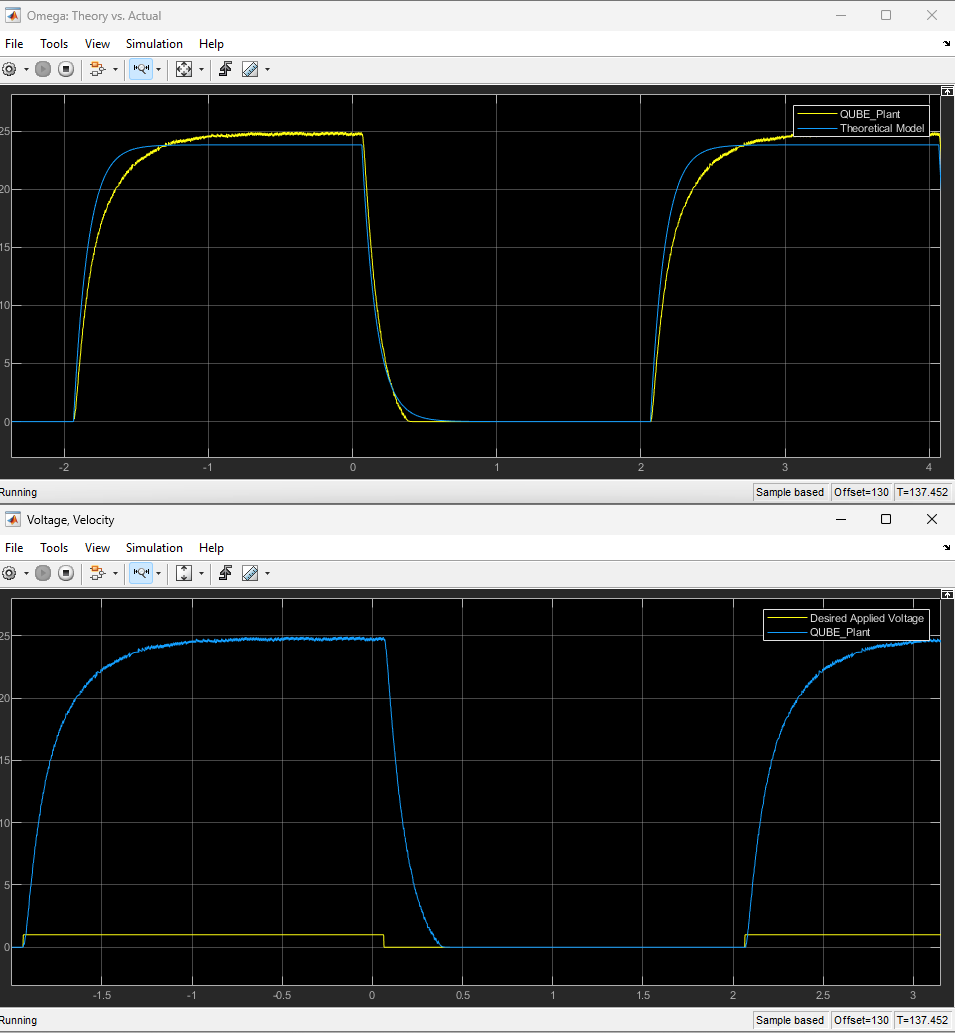
\includegraphics[width=0.5\textwidth]{1V.png}
\end{center}
\textbf{Input Voltage: 6 V}
\begin{center}
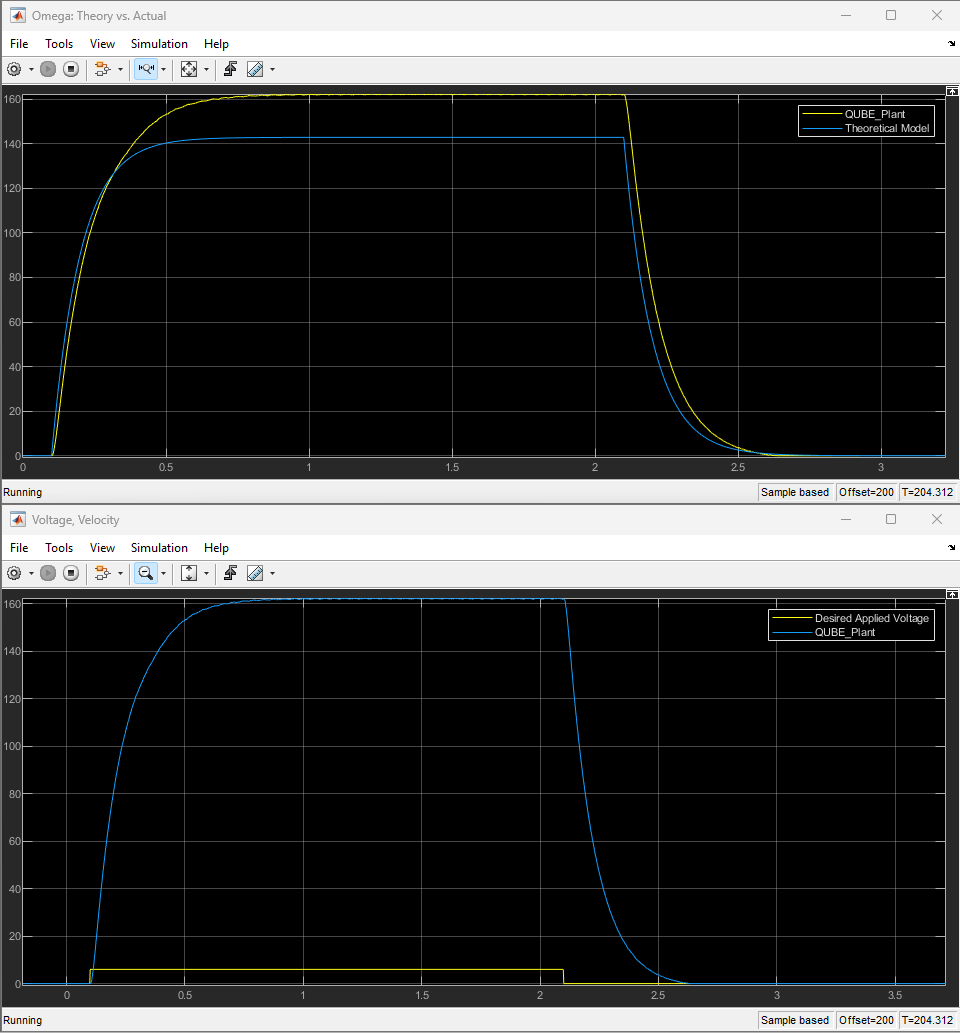
\includegraphics[width=0.5\textwidth]{6V.png}
\end{center}
\textbf{Input Voltage: 12 V}
\begin{center}
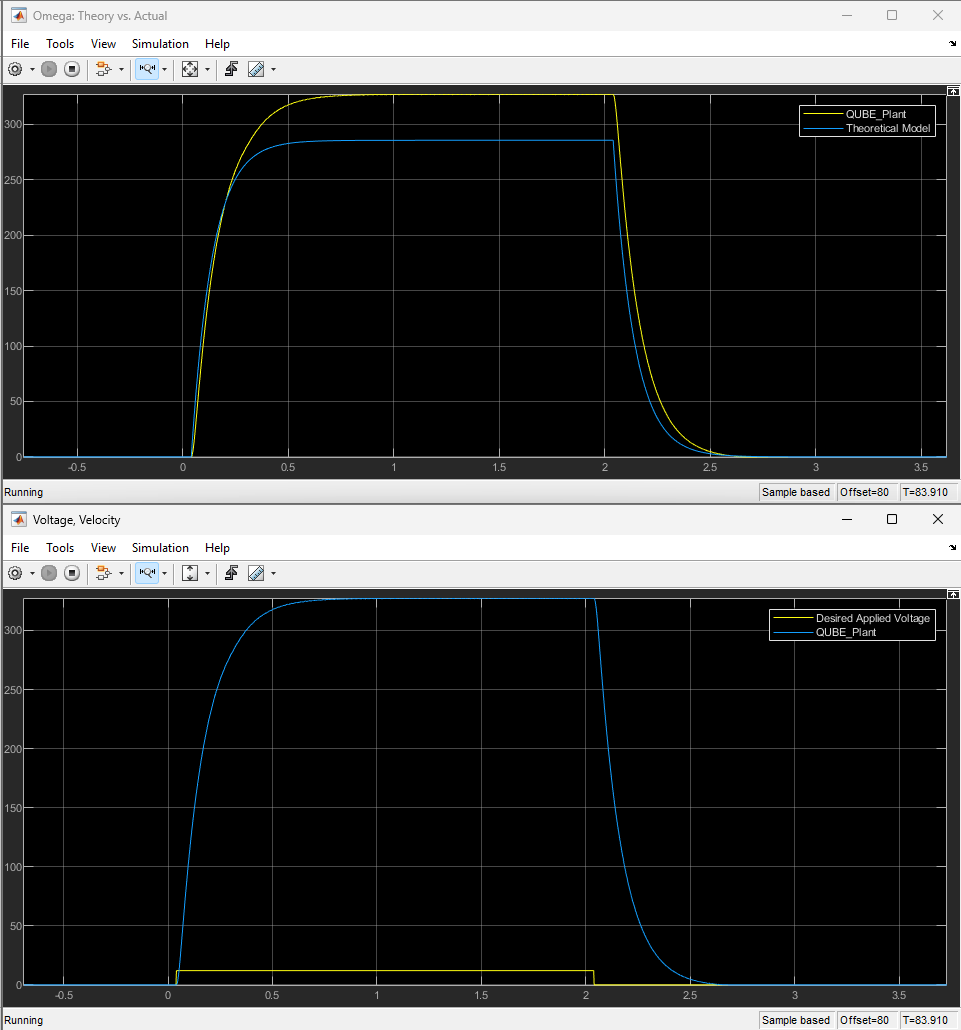
\includegraphics[width=0.5\textwidth]{12V.png}
\end{center}
\textbf{Input Voltage: 18 V}
\begin{center}
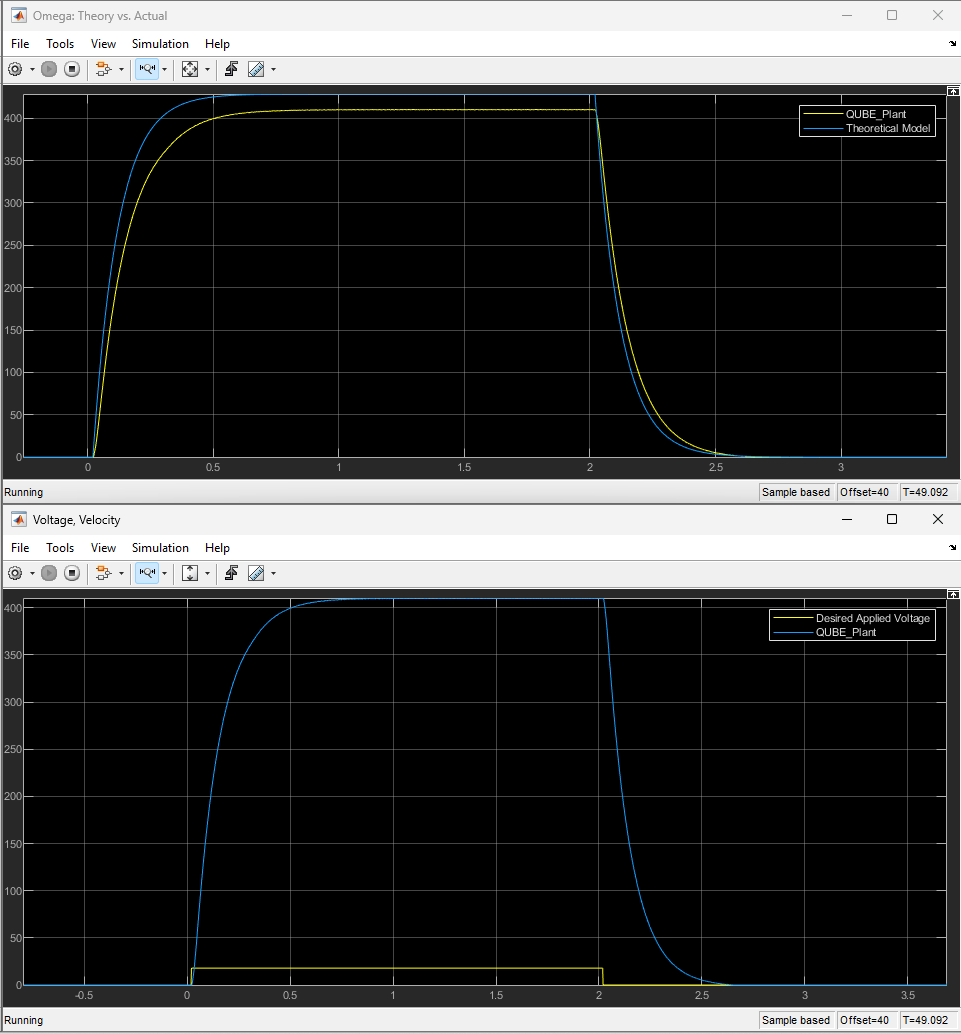
\includegraphics[width=0.5\textwidth]{18V.png}
\end{center}
\newpage\noindent
\textbf{Input Voltage: 20 V}
\begin{center}
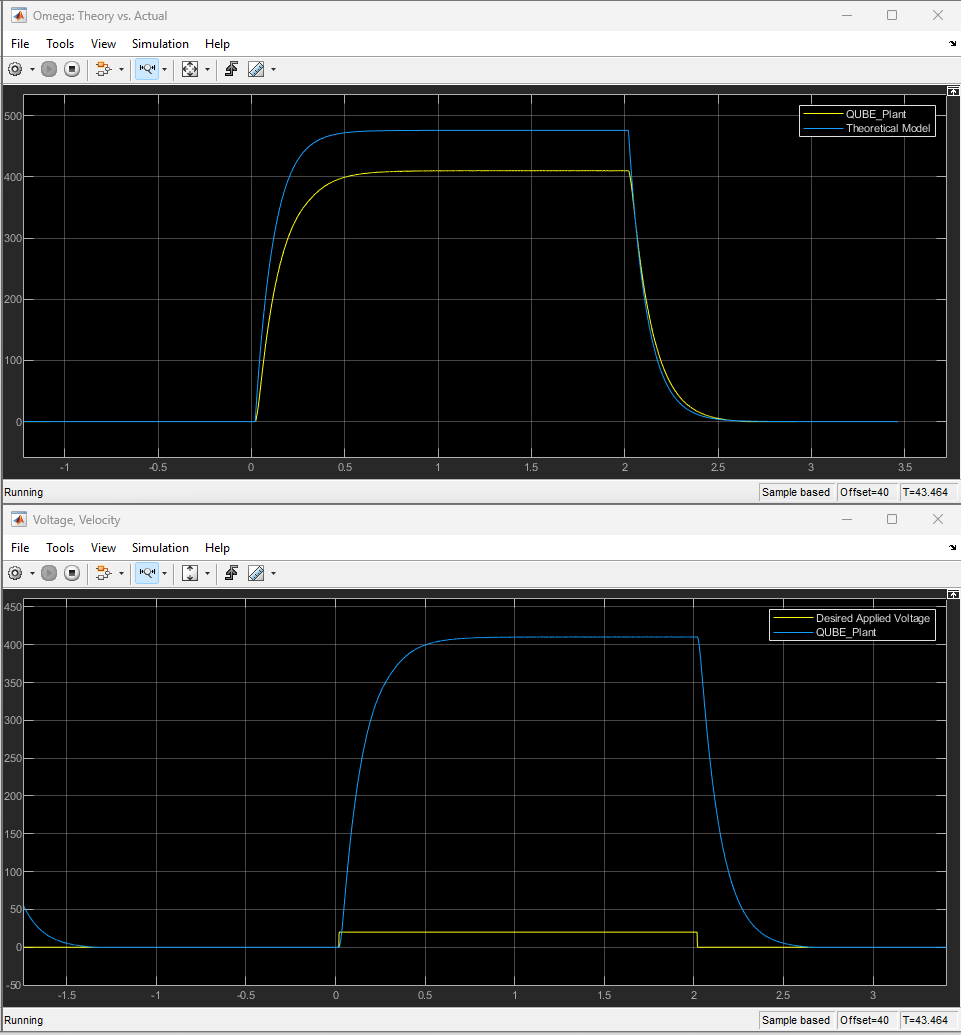
\includegraphics[width=0.5\textwidth]{20V.png}
\end{center}
\section*{Answers to Questions}
\begin{enumerate}
    \item At 6 V, the actual gain of the motor is higher than the theoretical gain and the theoretical model predicted a faster response than the actual response. Thus, the theoretical model has a smaller time constant than the actual motor.\\\\
    \textbf{Estimating the experimental time constant $\tau$}:\\
    For a 6V input, the steady state $\omega$ is about $1.625\times10^2$ rad/s. The time constant $\tau$ is the time it takes for the system to reach $63\%$ of the steady state value (102.375 rad/s). From the plot, the time taken to reach 102.375 rad/s is approximately 152.934 ms.
    \[\boxed{\tau_\text{experimental} = 0.152934 \,\text{s}}\]
    This is indeed larger than the theoretical time constant of 0.0997 s.\\\\
    \textbf{Estimating the experimental DC gain $K$}:\\
    The steady state output for a unit step input of 1 V is 24.87 rad/s. 
    \[\boxed{K_\text{experimental} = 24.87 \,\text{(rad/s)/V}}\]
    This is also higher than the theoretical gain of 23.809 (rad/s)/V.
    \item Generally, the theoretical model is quite bad at predicting the forced step response, however it matches quite well for the free response after the step input is removed. The forced step response differs between voltages in that the DC gain is not consistently higher or lower than the theoretical model. However, the theoretical model consistently predicts a faster response than the actual motor, which means the theoretical time constant is smaller.
    \item At lower voltages (1,6, and 12 V), the theoretical model had a smaller DC gain than the actual motor, but this is flipped for higher voltages (18 and 20 V). 
    \item As previously mentioned, the theoretical time constant is consistently smaller than the experimental time constant, and the DC gain compared to the actual motor is smaller at lower voltages but larger at higher voltages. 
\end{enumerate}



\end{document}
